\chapter{Event Selection}
\label{chap:Evt}

Events are required to contain exactly two \emph{tight} leptons and one \emph{tight} hadronic tau. A combination of single- and di-lepton triggers are used to select events.
%%%%%%%%%%%%%%%%%%%%%%%%%%%%%%%%%%%%%%%%%%%%%%%%%%
%%%%%%%%%%%%%%%%%%%%%%%%%%%%%%%%%%%%%%%%%%%%%%%%%%
\section{Event Categorization}
\label{sec:Cat}

\begin{figure}[tbh!]
 \begin{center}
 \begin{tabular}{c}
 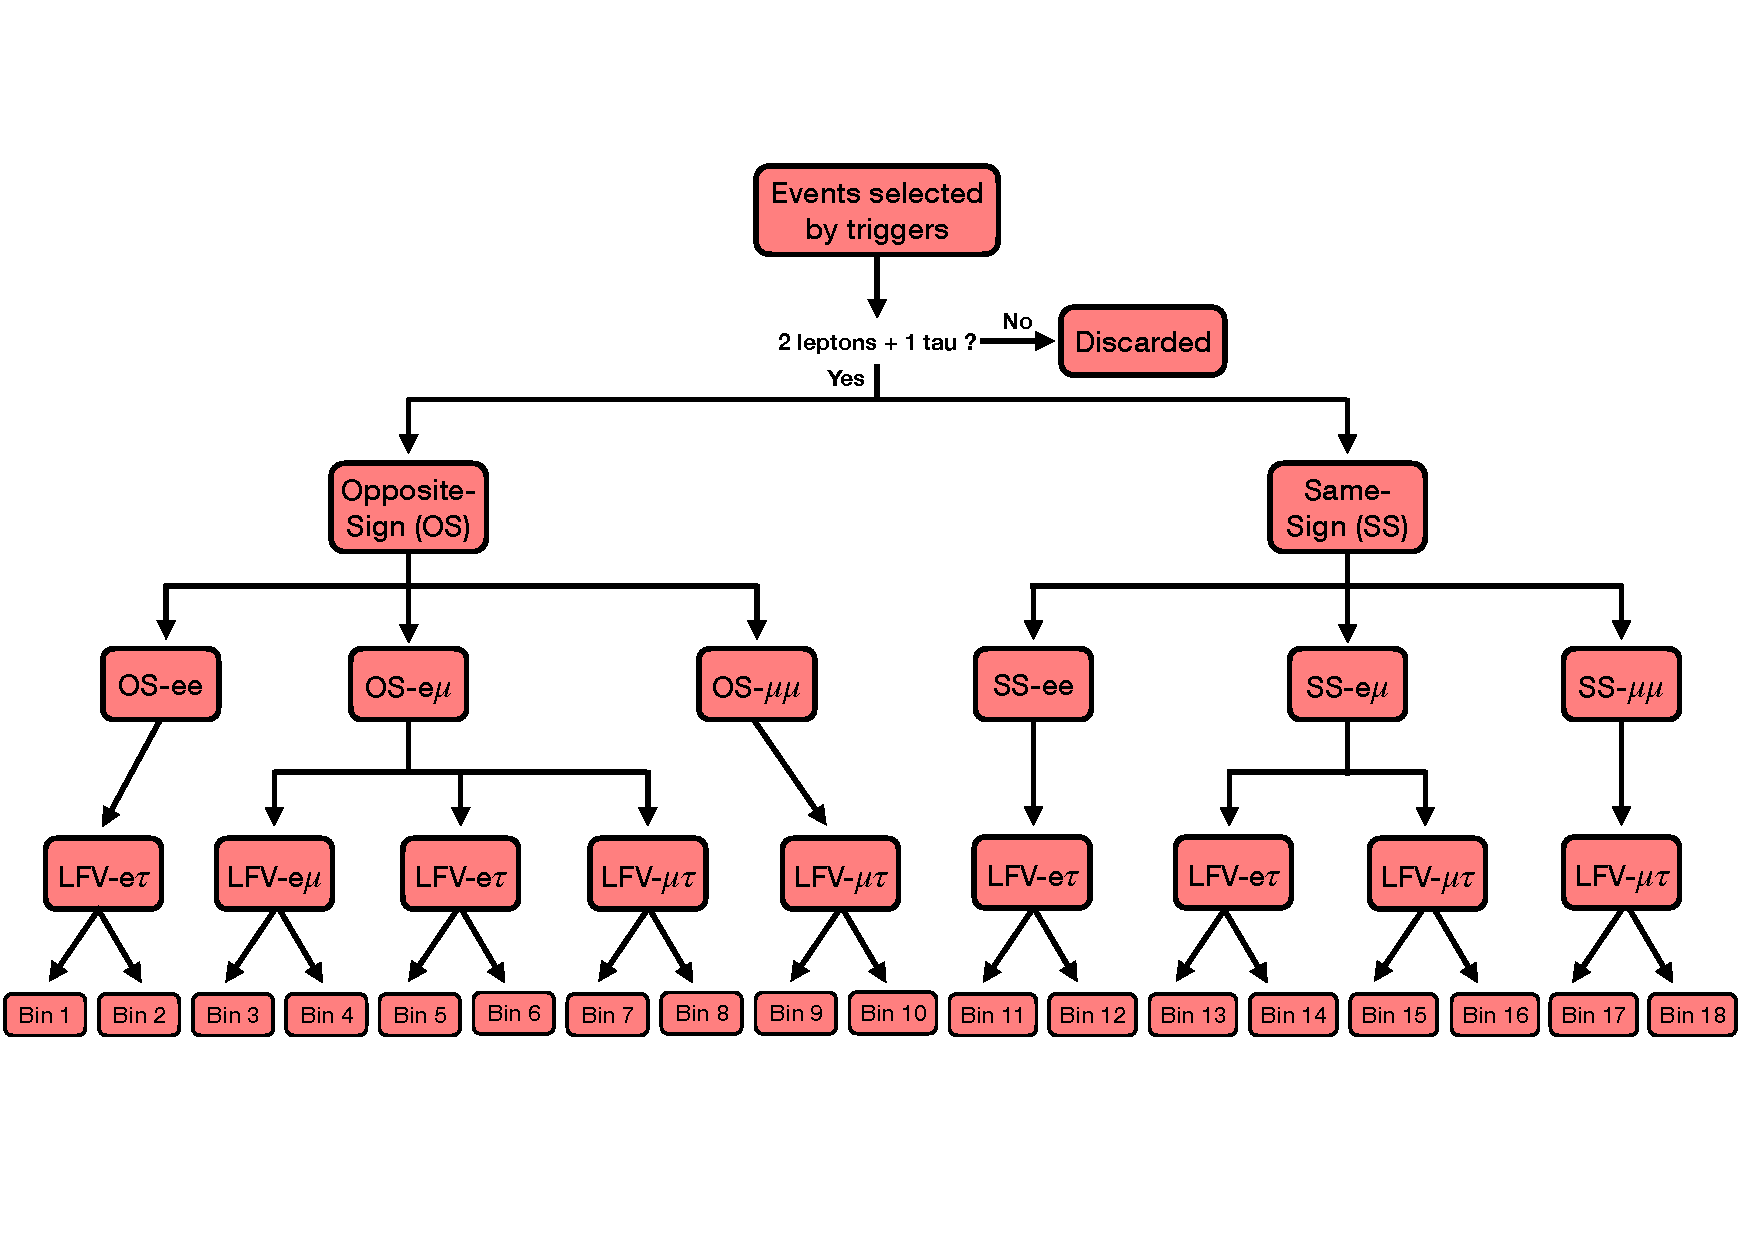
\includegraphics[width=\textwidth]{figures/Part4/Evt/SRFlowChart}
 \end{tabular}
 \caption{XX}
 \label{fig:EvtCat}
 \end{center}
 \end{figure}
%%%%%%%%%%%%%%%%%%%%%%%%%%%%%%%%%%%%%%%%%%%%%%%%%%
%%%%%%%%%%%%%%%%%%%%%%%%%%%%%%%%%%%%%%%%%%%%%%%%%%

\section{Signal Region}
\label{sec:SRInclusive}

\begin{figure}[tbh!]
 \begin{center}
 \begin{tabular}{c}
 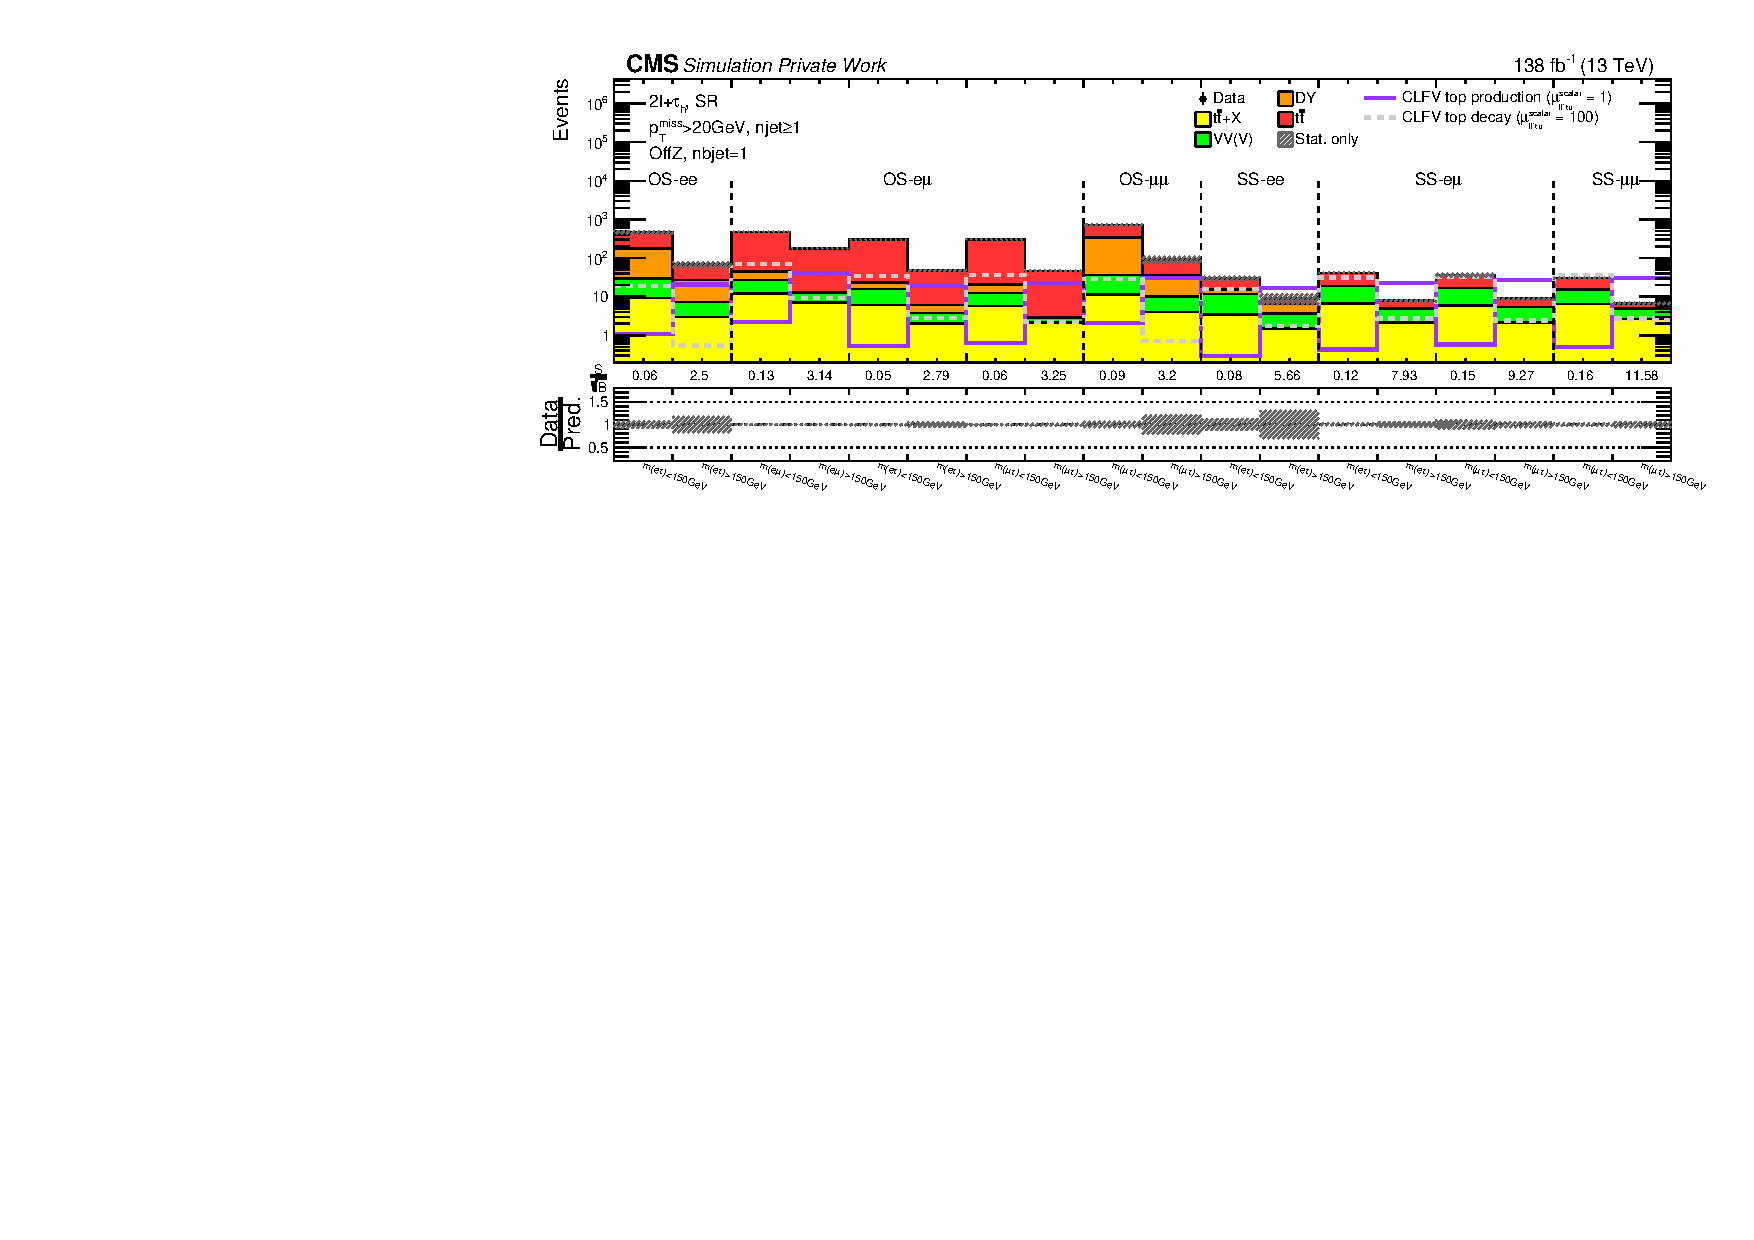
\includegraphics[width=\textwidth]{figures/Part4/Evt/Summary_llOffZMetg20B1}
 \end{tabular}
 \caption{XX}
 \label{fig:Summary}
 \end{center}
 \end{figure}
 
 \begin{figure}[tbh!]
 \begin{center}
 \begin{tabular}{c}
 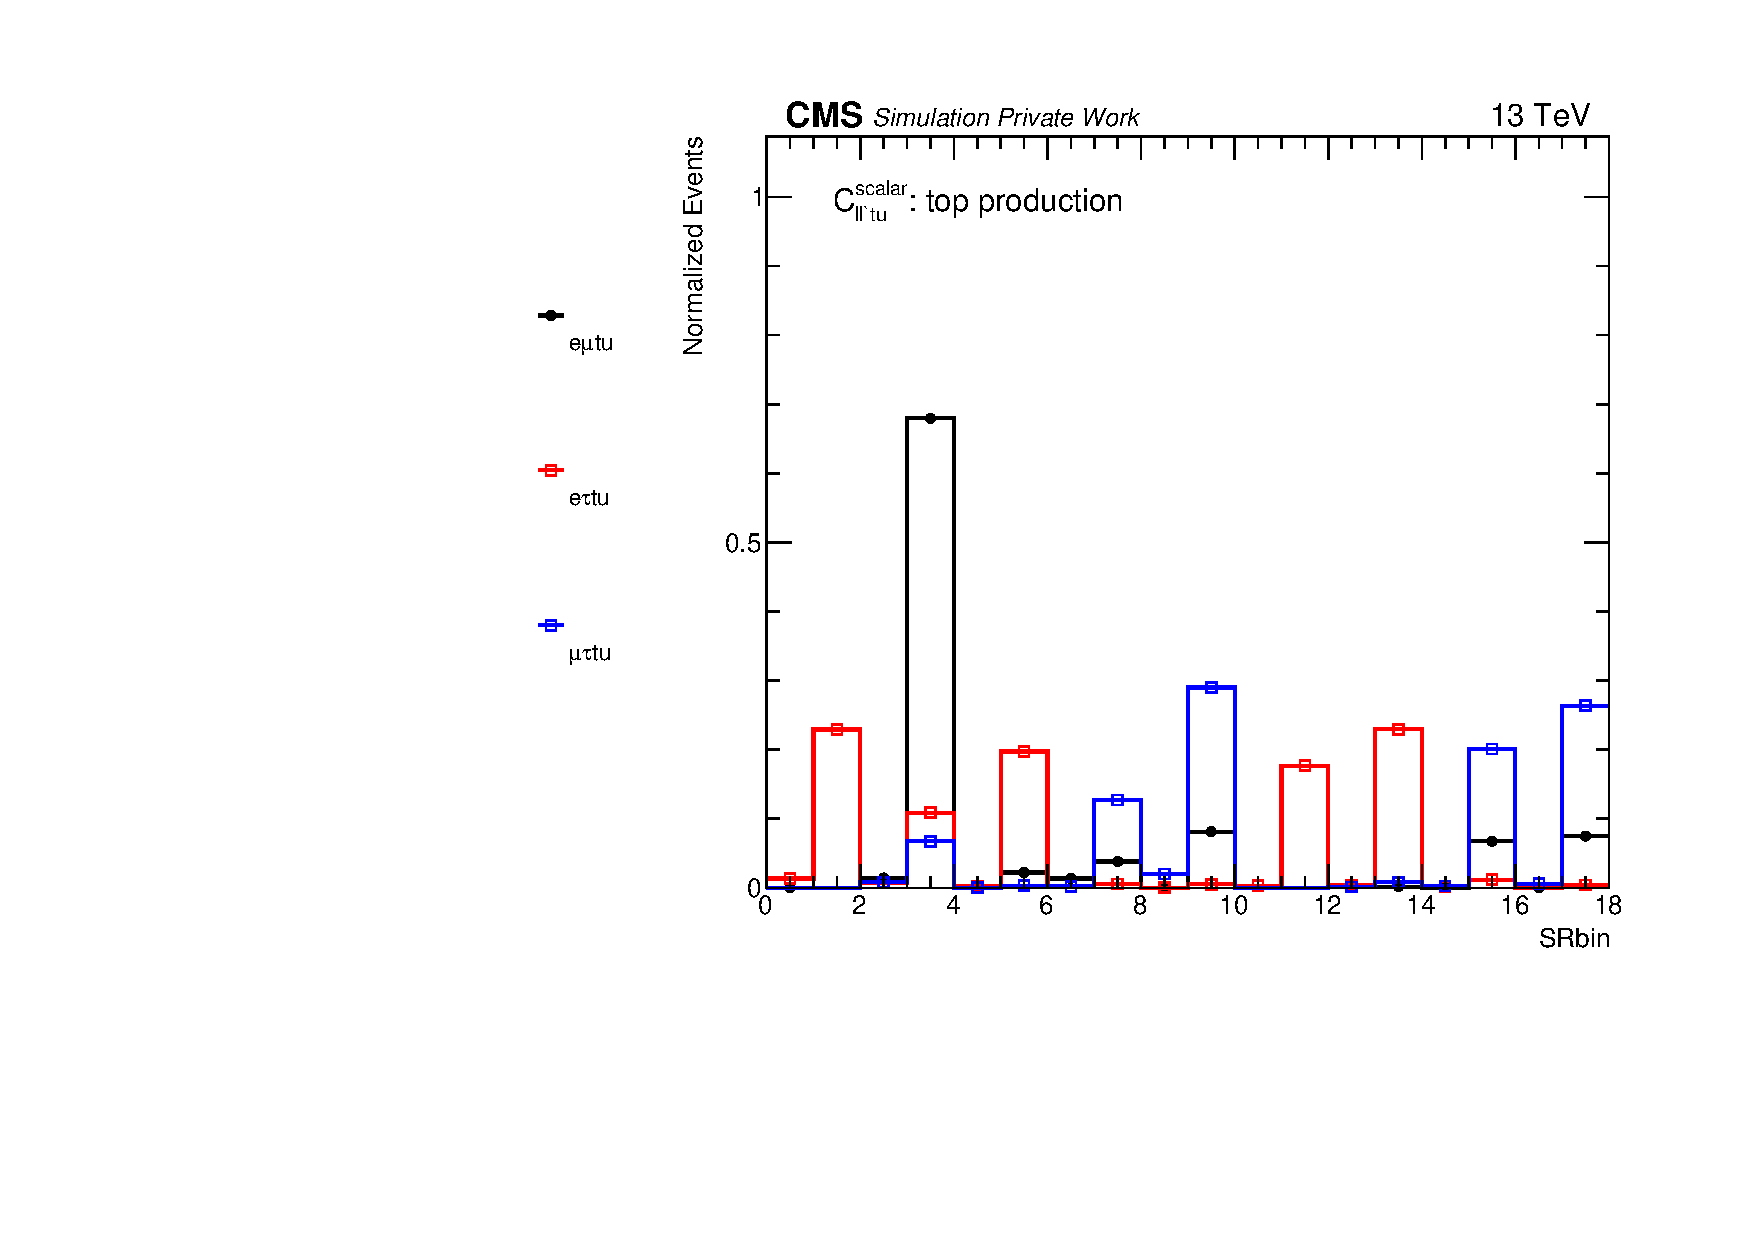
\includegraphics[width=\textwidth]{figures/Part4/Evt/SRbin}
 \end{tabular}
 \caption{XX}
 \label{fig:SRbin}
 \end{center}
 \end{figure}
 
 \begin{figure}[tbh!]
 \begin{center}
 \begin{tabular}{ccc}
 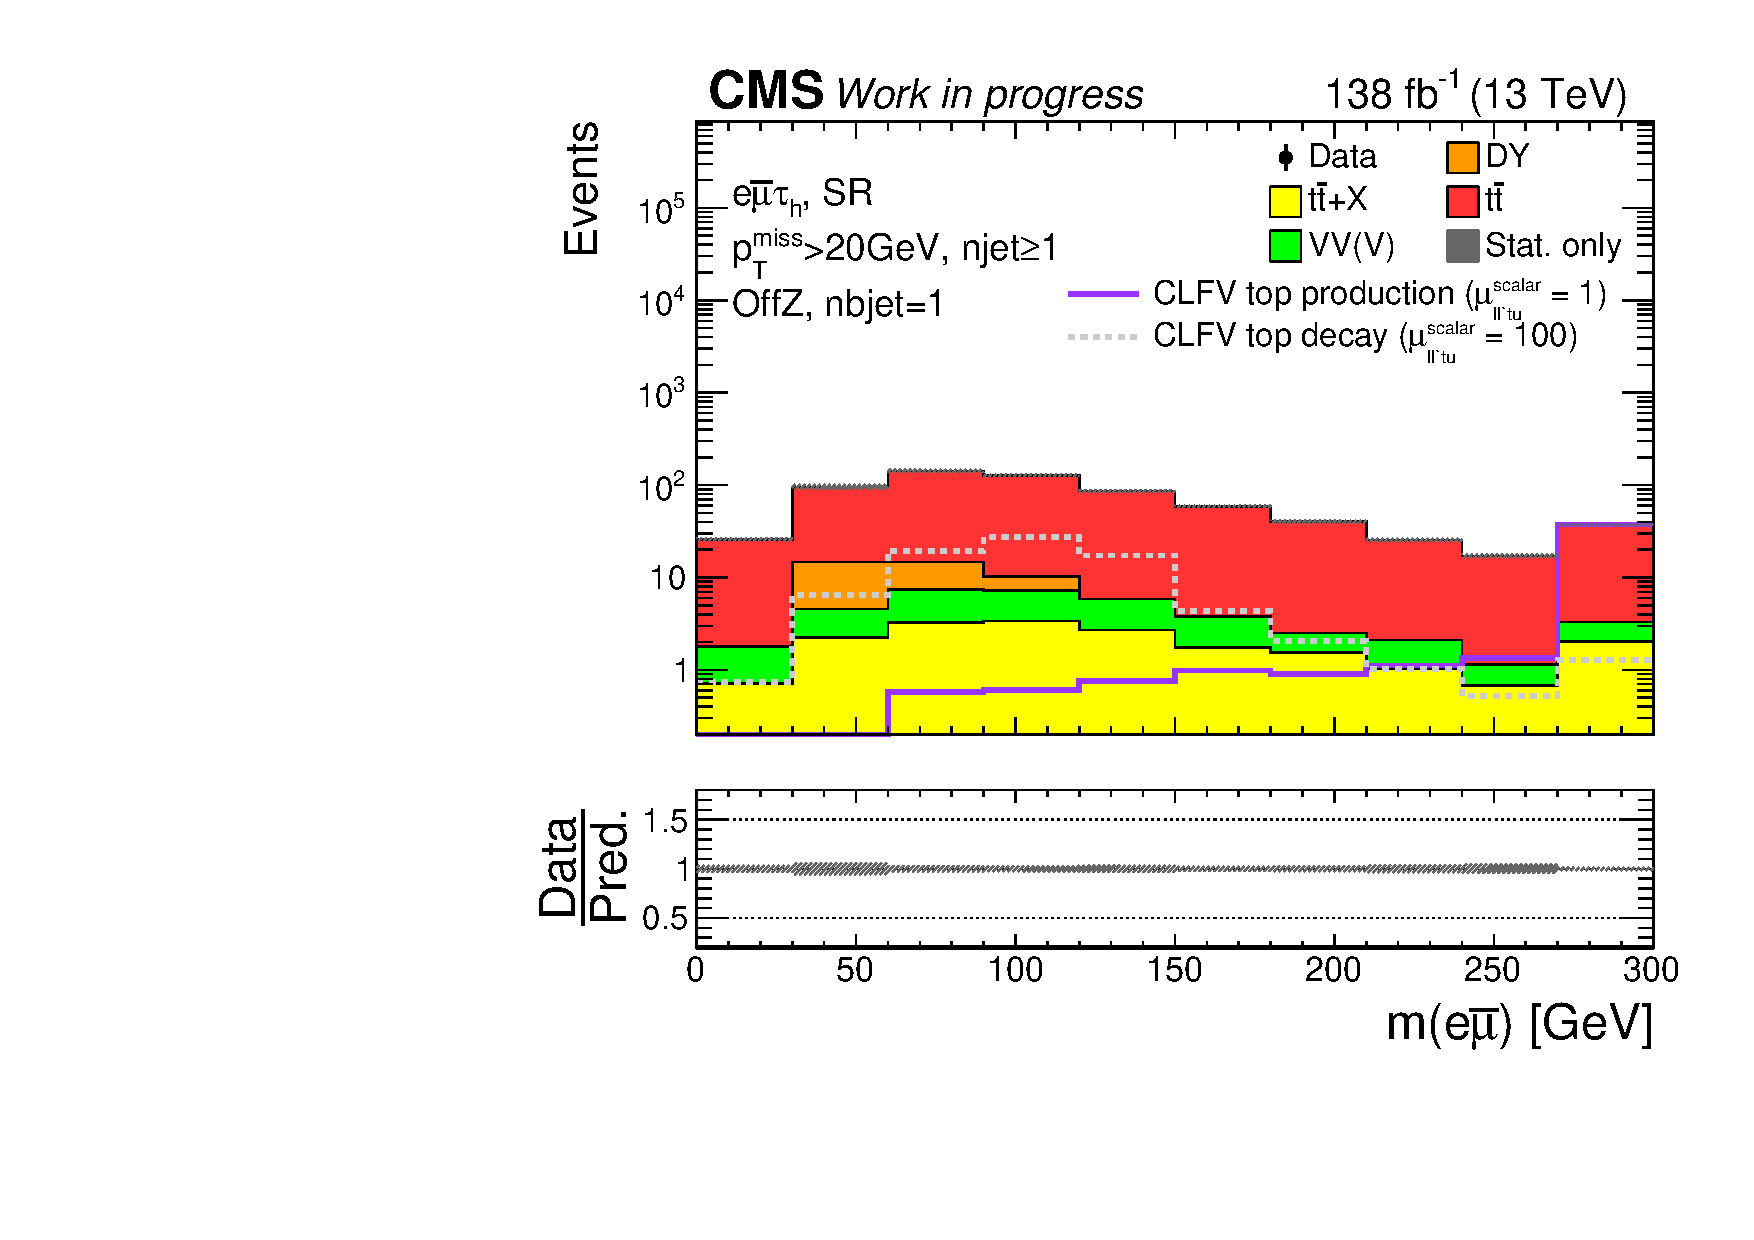
\includegraphics[width=0.33\textwidth]{figures/Part4/Evt/LFVemuM}&
 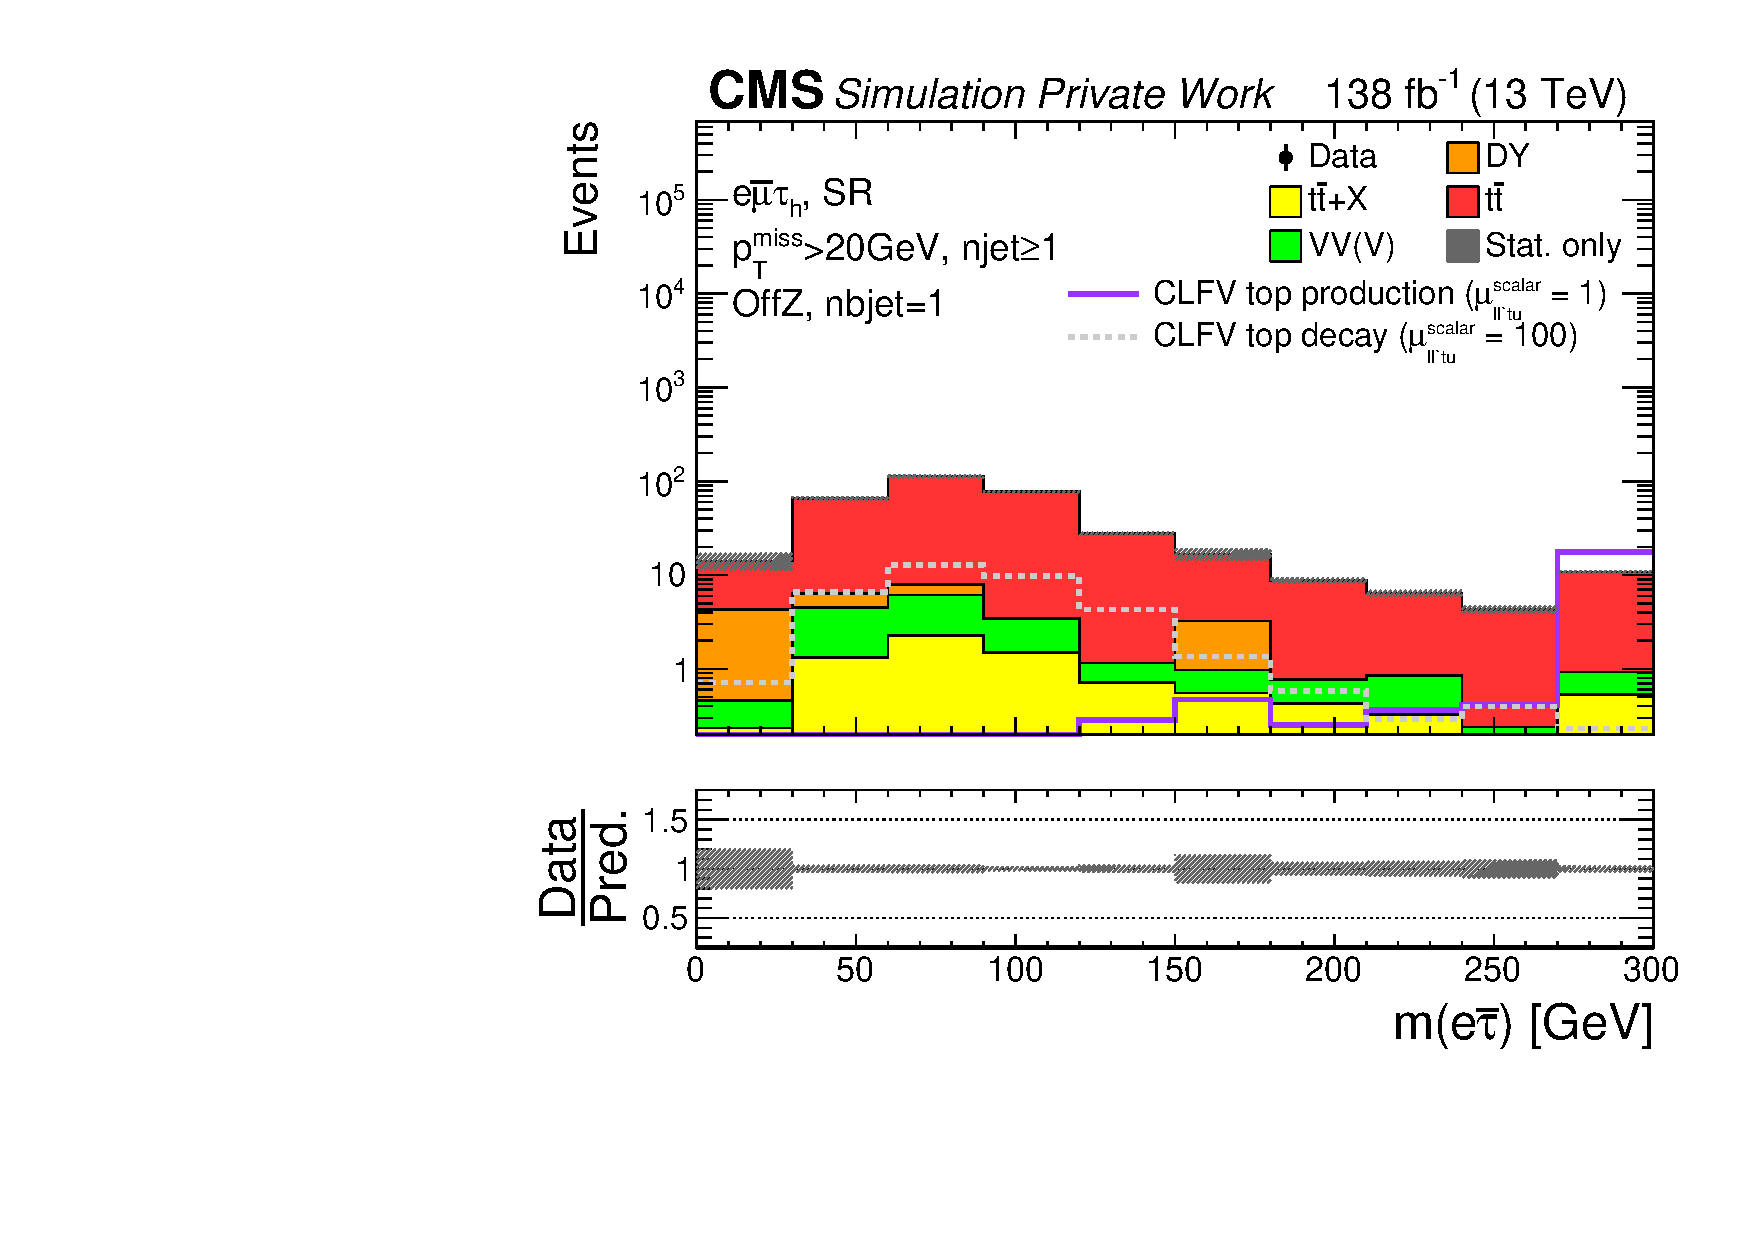
\includegraphics[width=0.33\textwidth]{figures/Part4/Evt/LFVetaM}&
 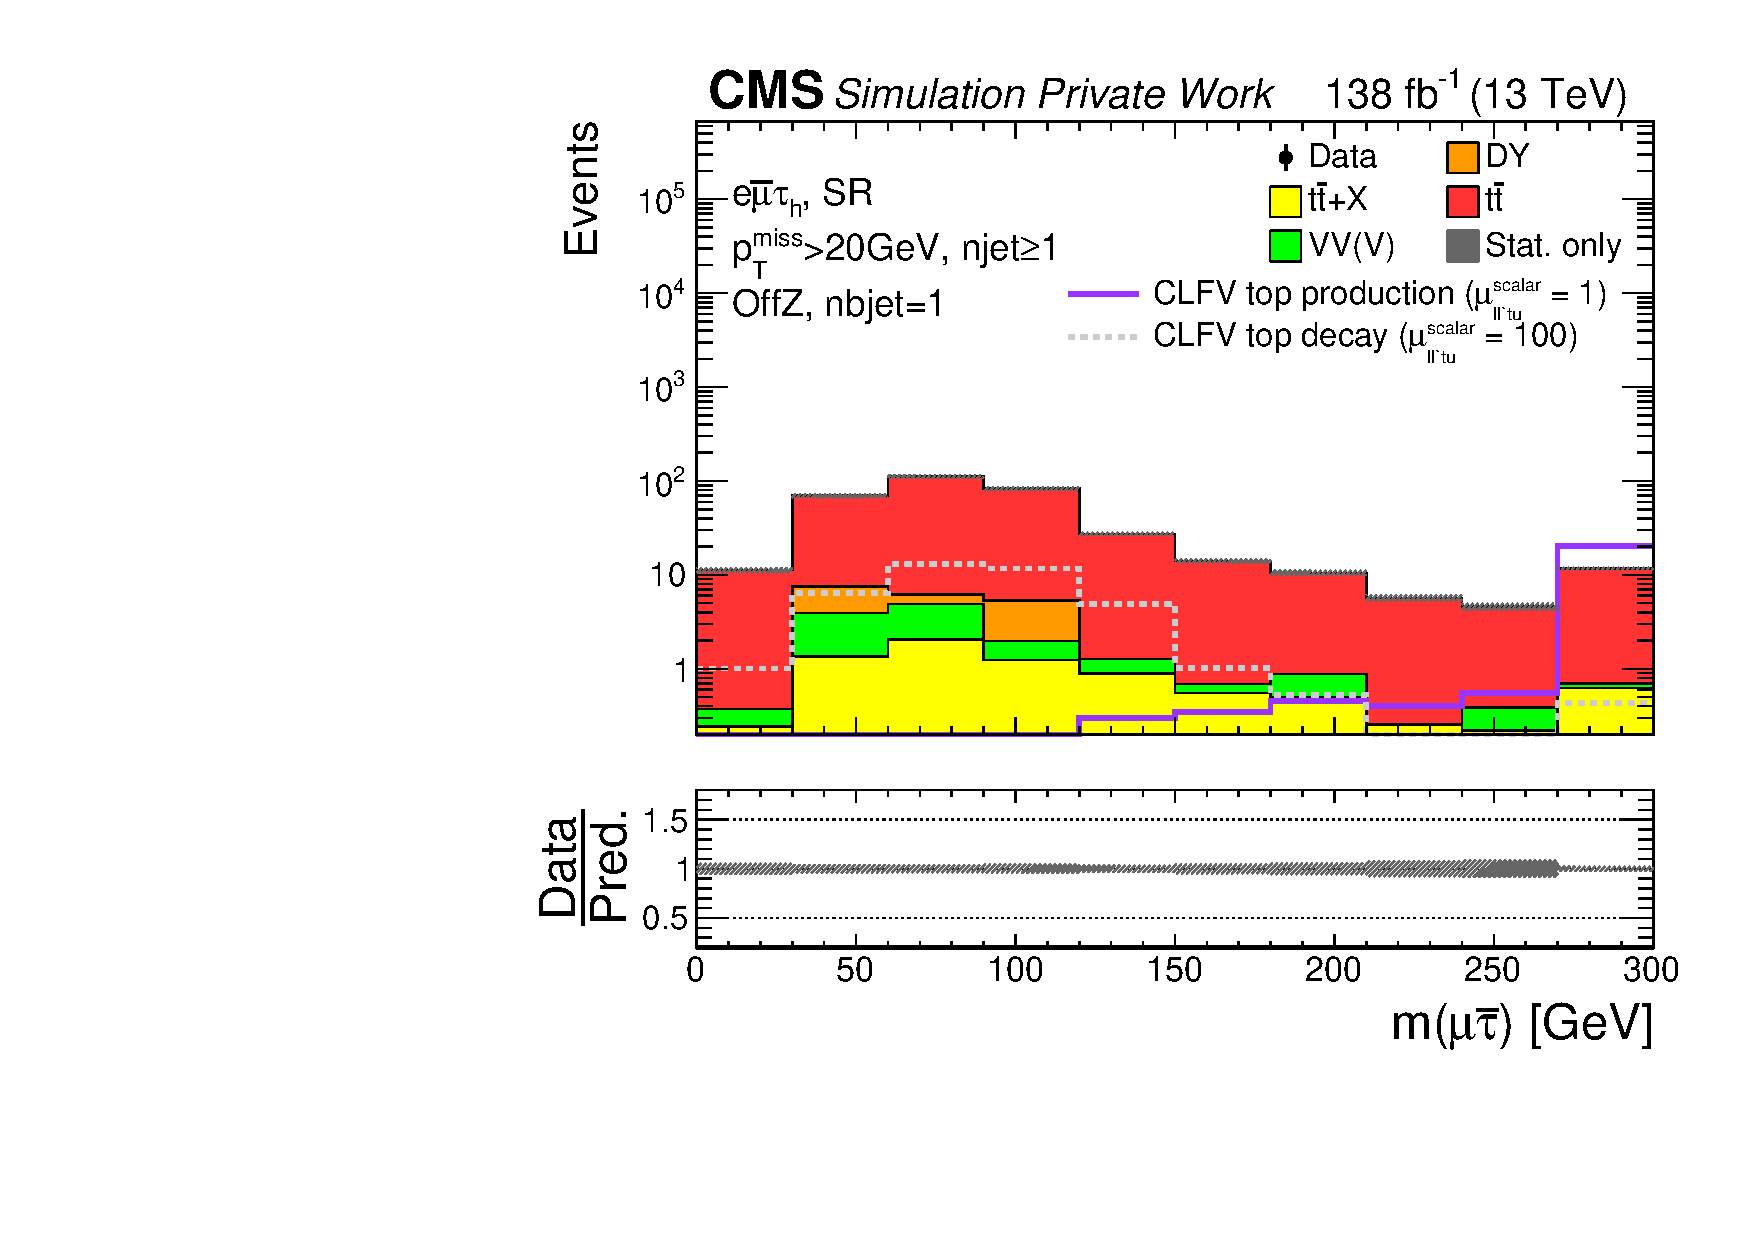
\includegraphics[width=0.33\textwidth]{figures/Part4/Evt/LFVmutaM}\\
 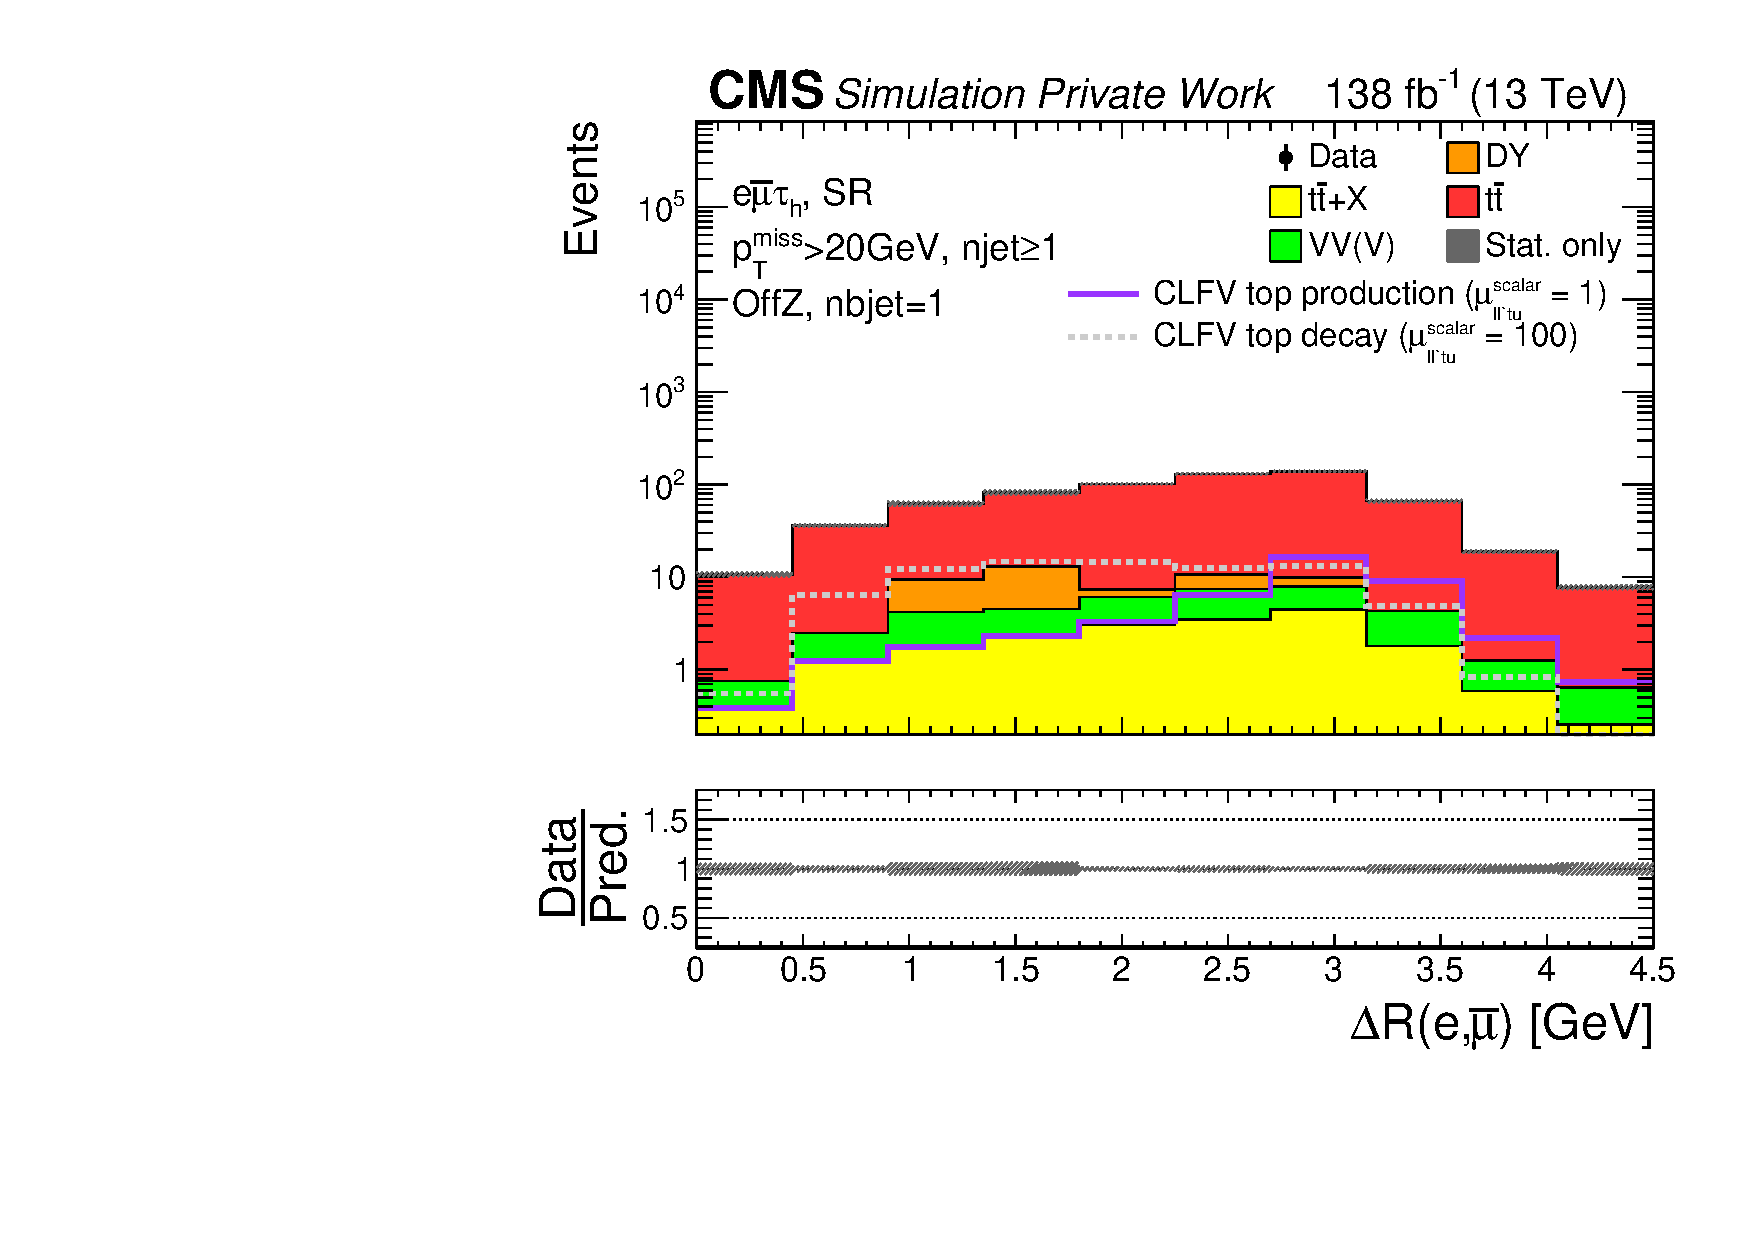
\includegraphics[width=0.33\textwidth]{figures/Part4/Evt/LFVemuDr}&
 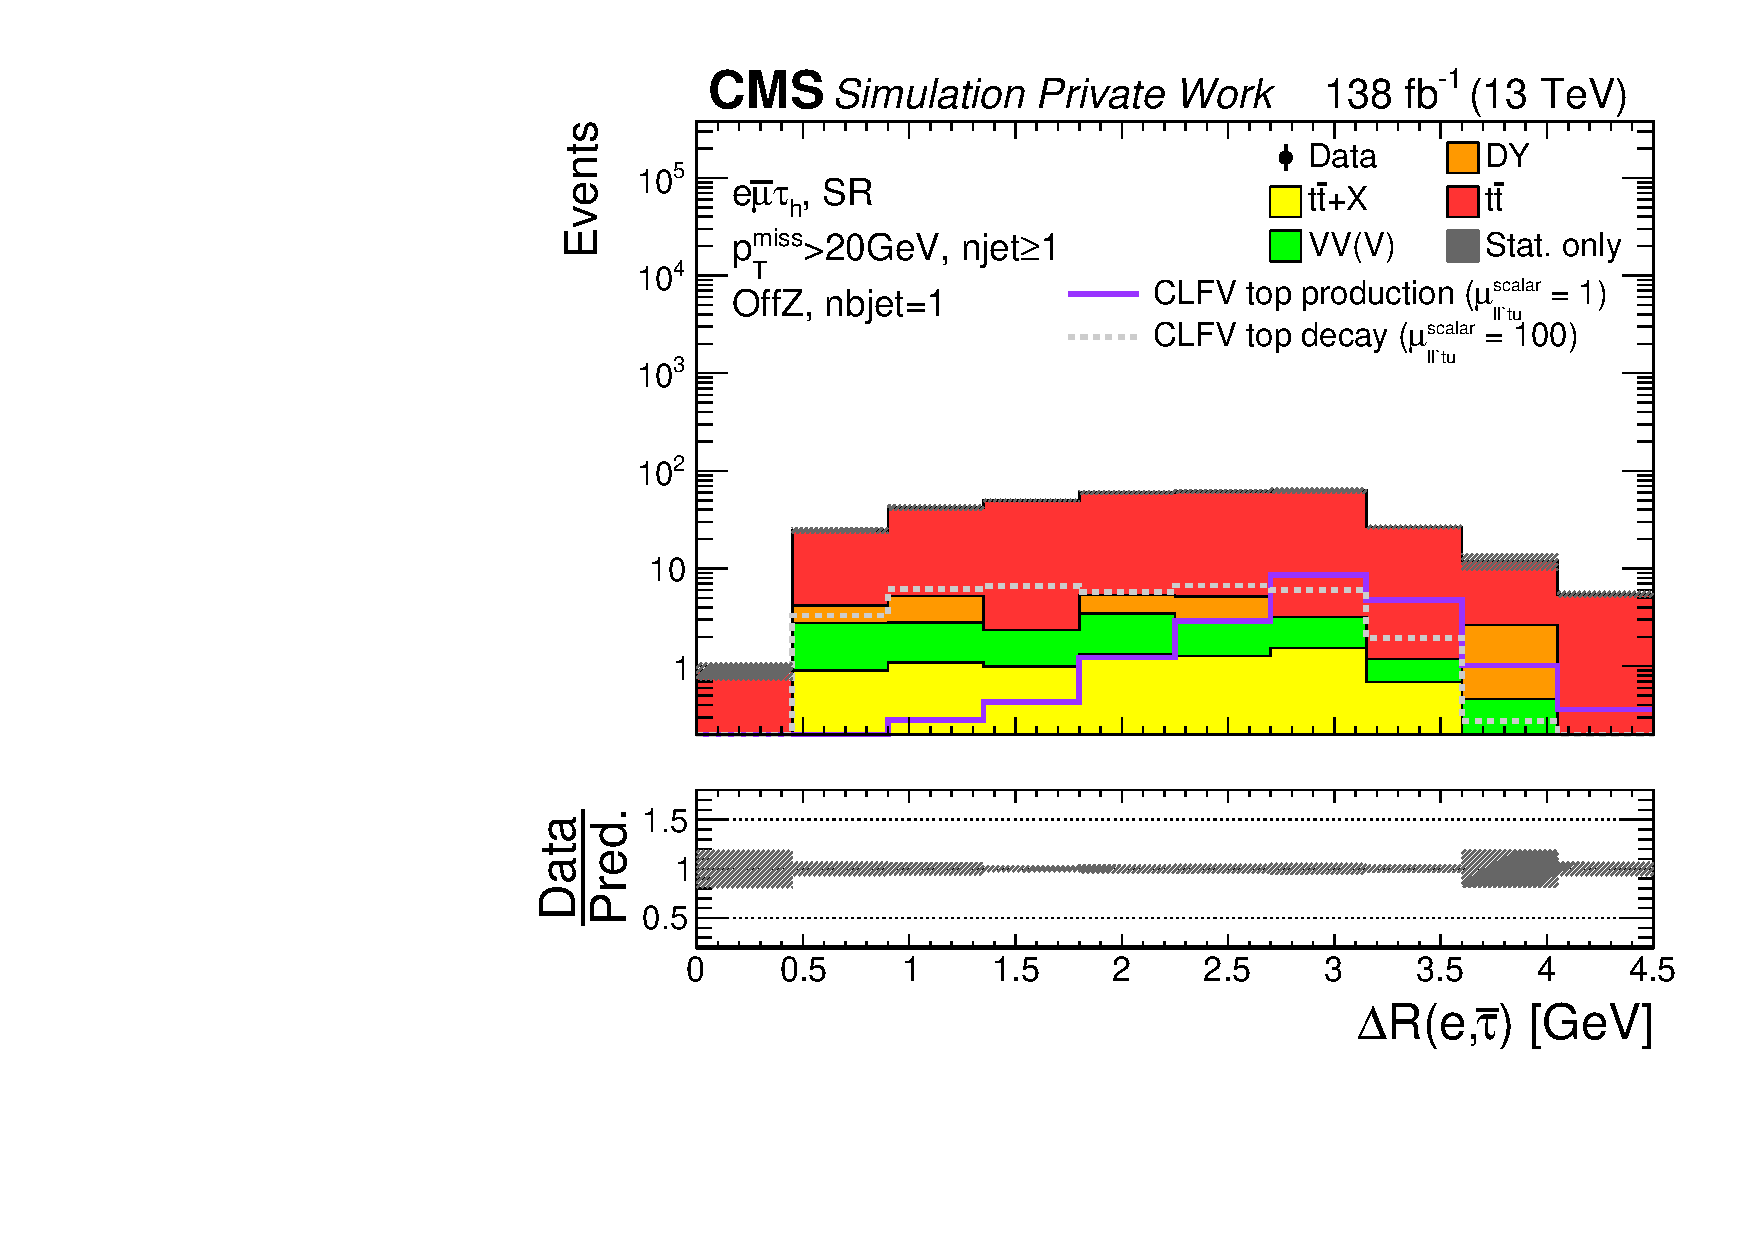
\includegraphics[width=0.33\textwidth]{figures/Part4/Evt/LFVetaDr}&
 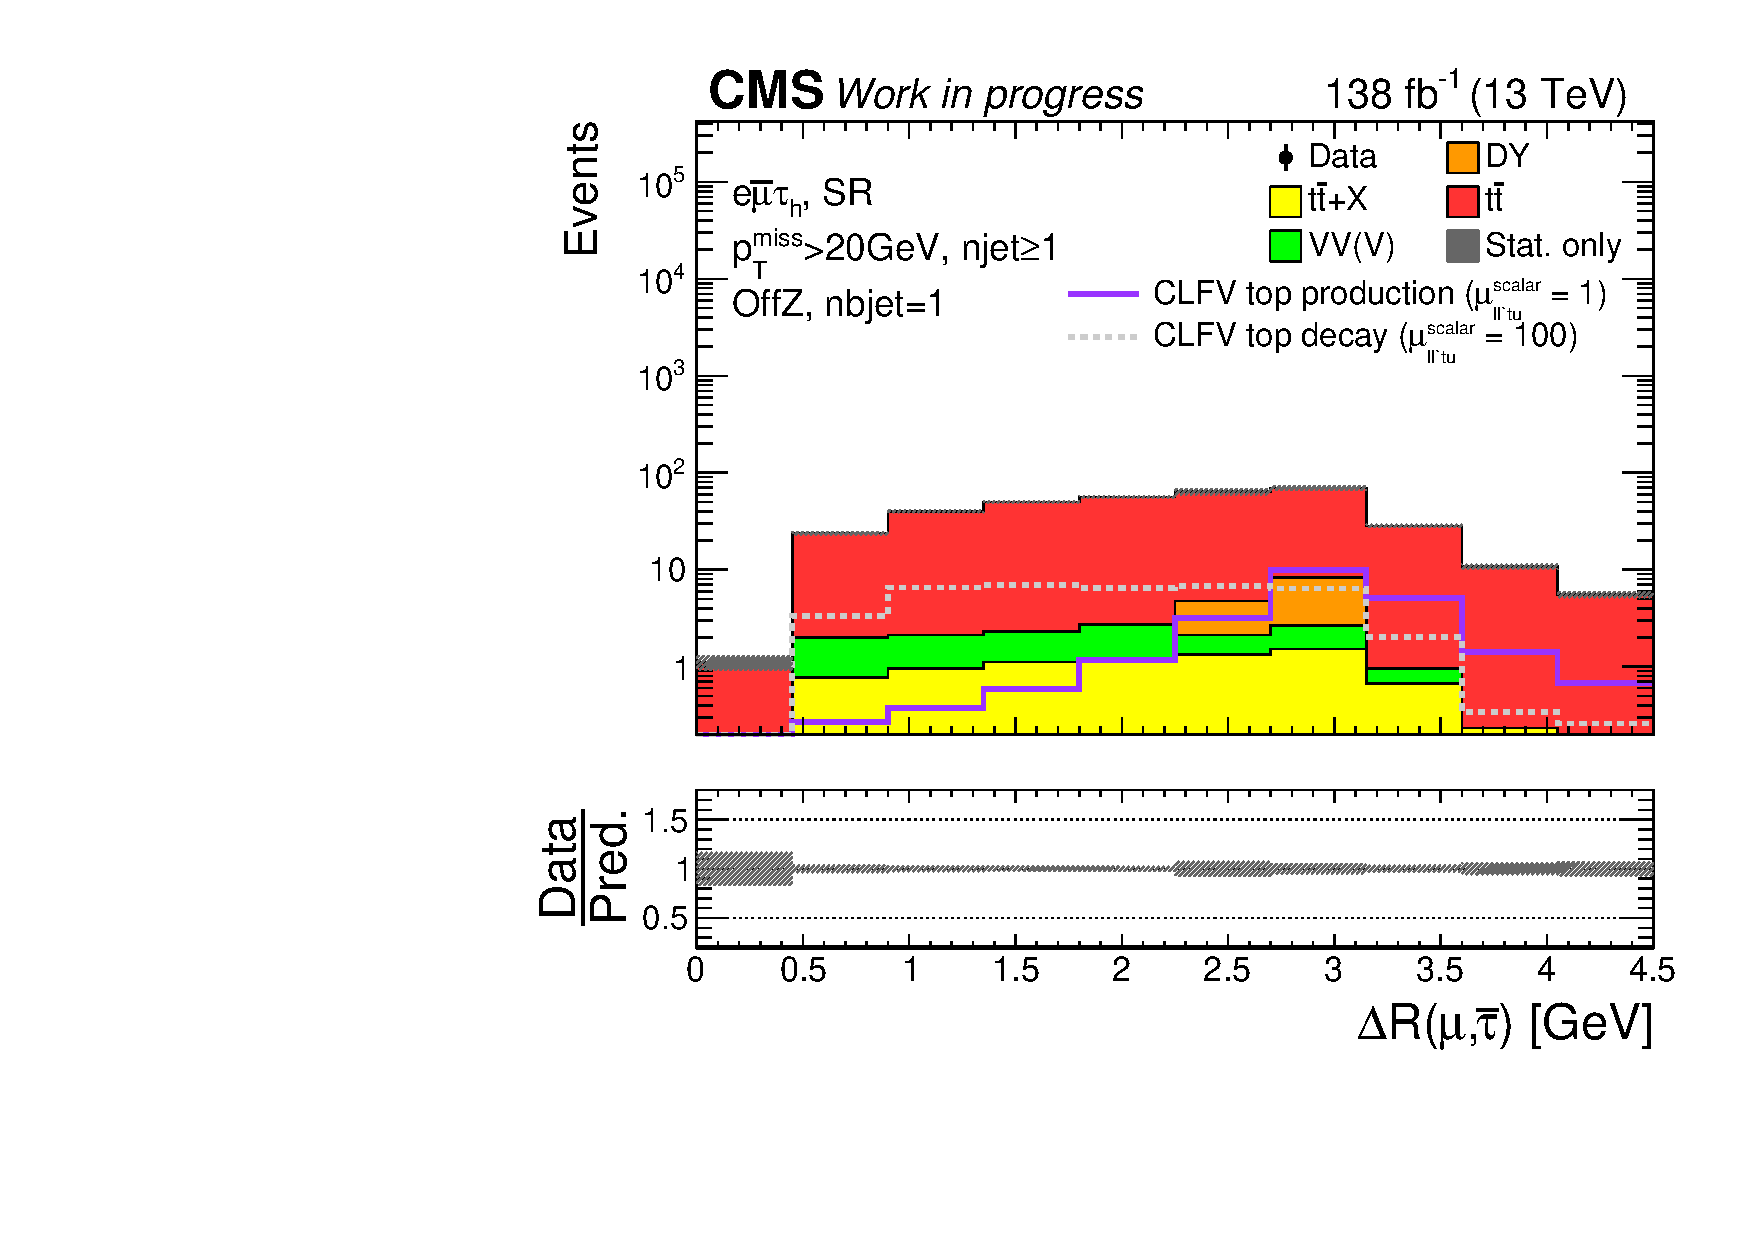
\includegraphics[width=0.33\textwidth]{figures/Part4/Evt/LFVmutaDr}\\
 \end{tabular}
 \caption{XX}
 \label{fig:LFVmass}
 \end{center}
 \end{figure}
%%%%%%%%%%%%%%%%%%%%%%%%%%%%%%%%%%%%%%%%%%%%%%%%%%
%%%%%%%%%%%%%%%%%%%%%%%%%%%%%%%%%%%%%%%%%%%%%%%%%%

\section{Drell-Yan Control Region}
\label{sec:DY_CR}

 \begin{figure}[tbh!]
 \begin{center}
 \begin{tabular}{cc}
 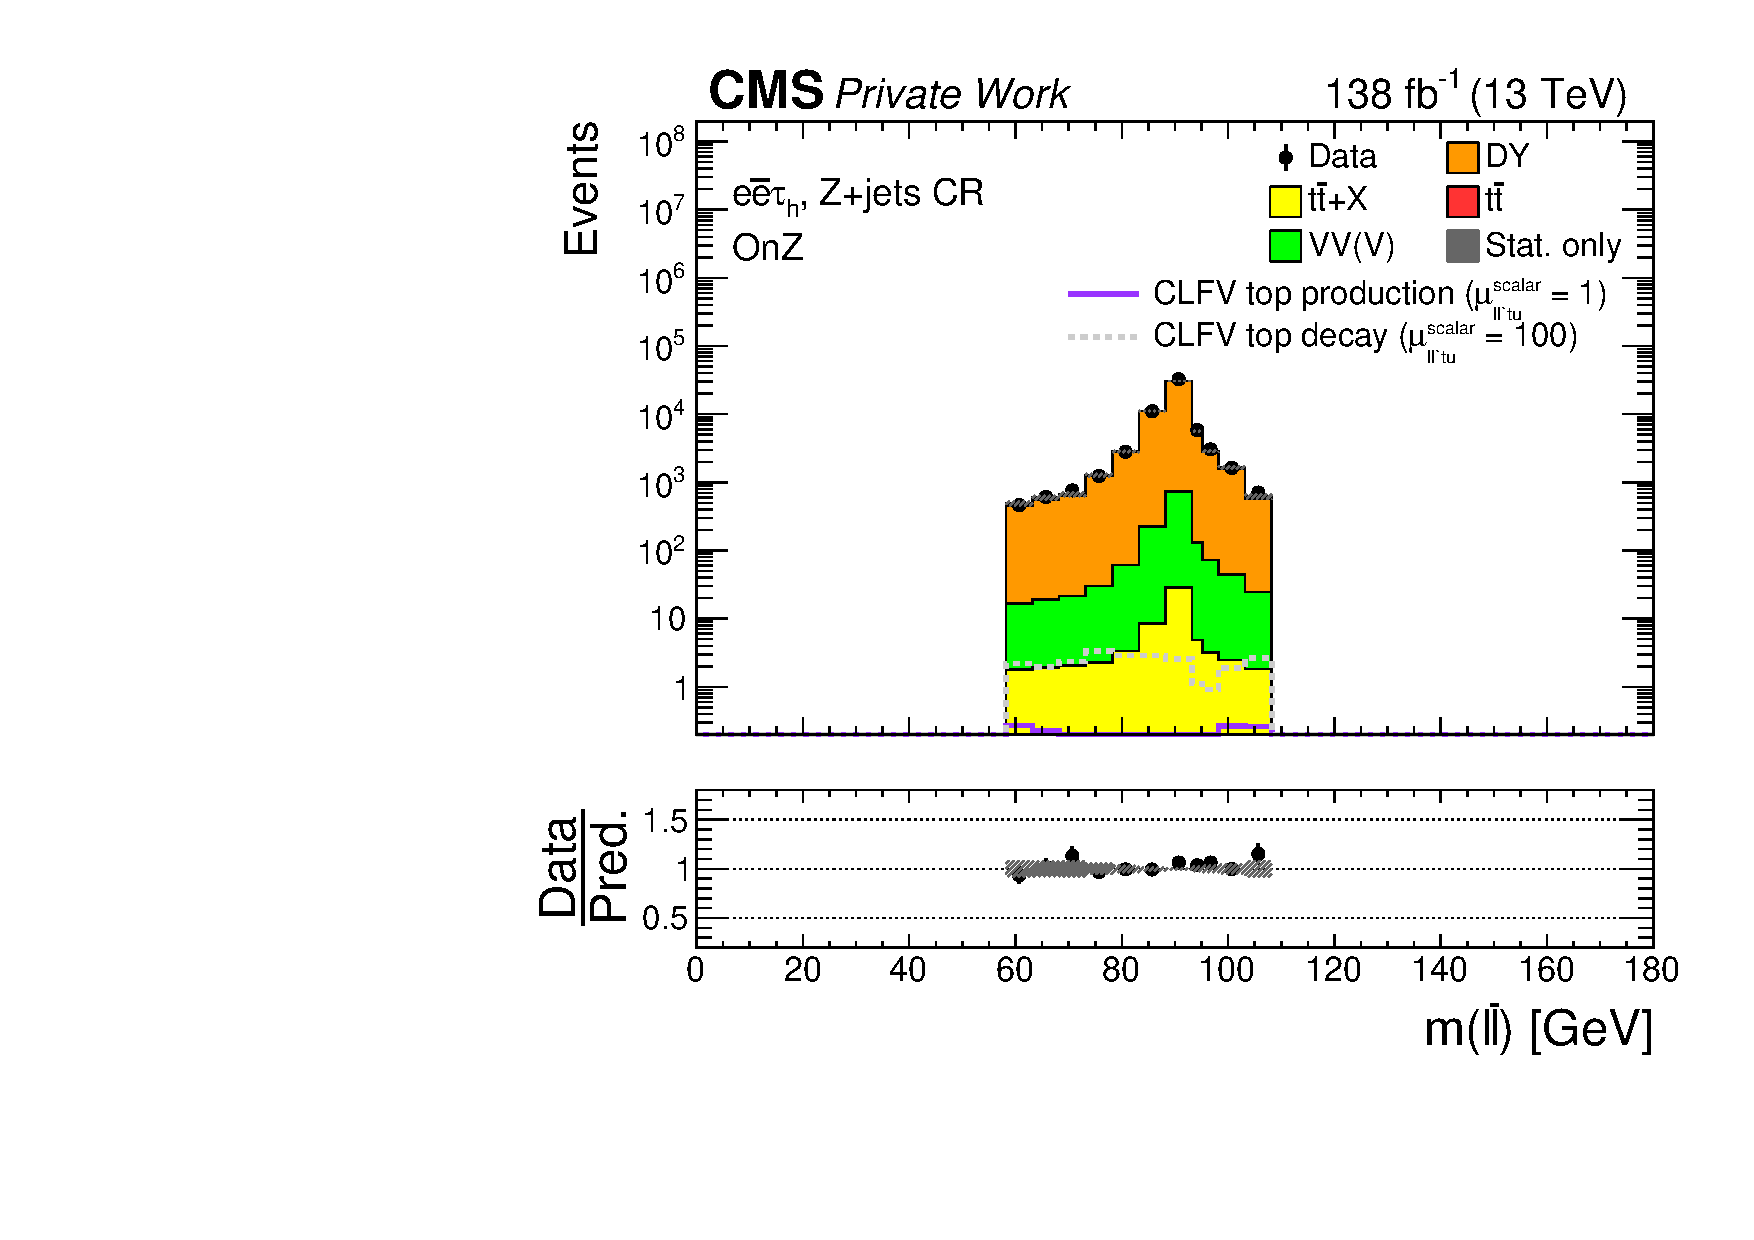
\includegraphics[width=0.48\textwidth]{figures/Part4/Evt/llM_OnZ_ee}&
 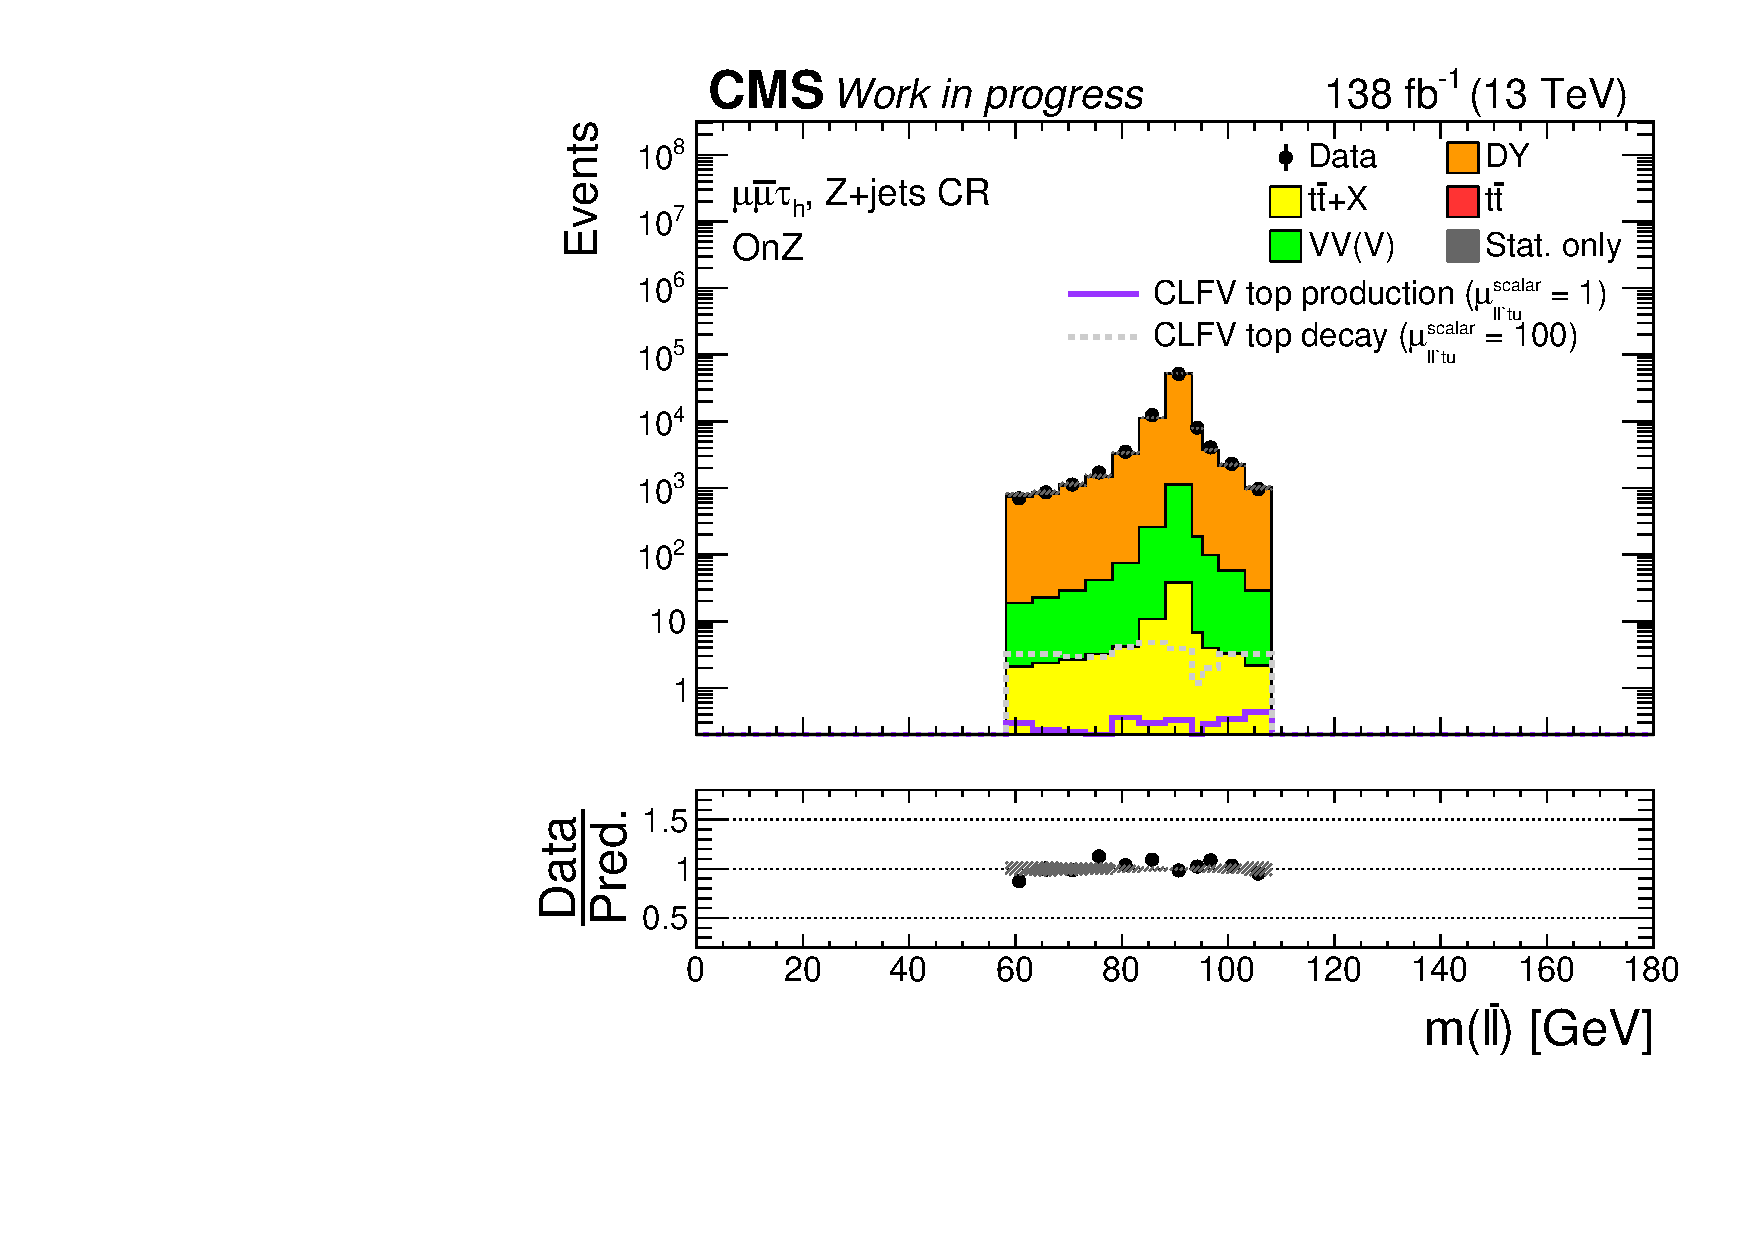
\includegraphics[width=0.48\textwidth]{figures/Part4/Evt/llM_OnZ_mumu}\\
  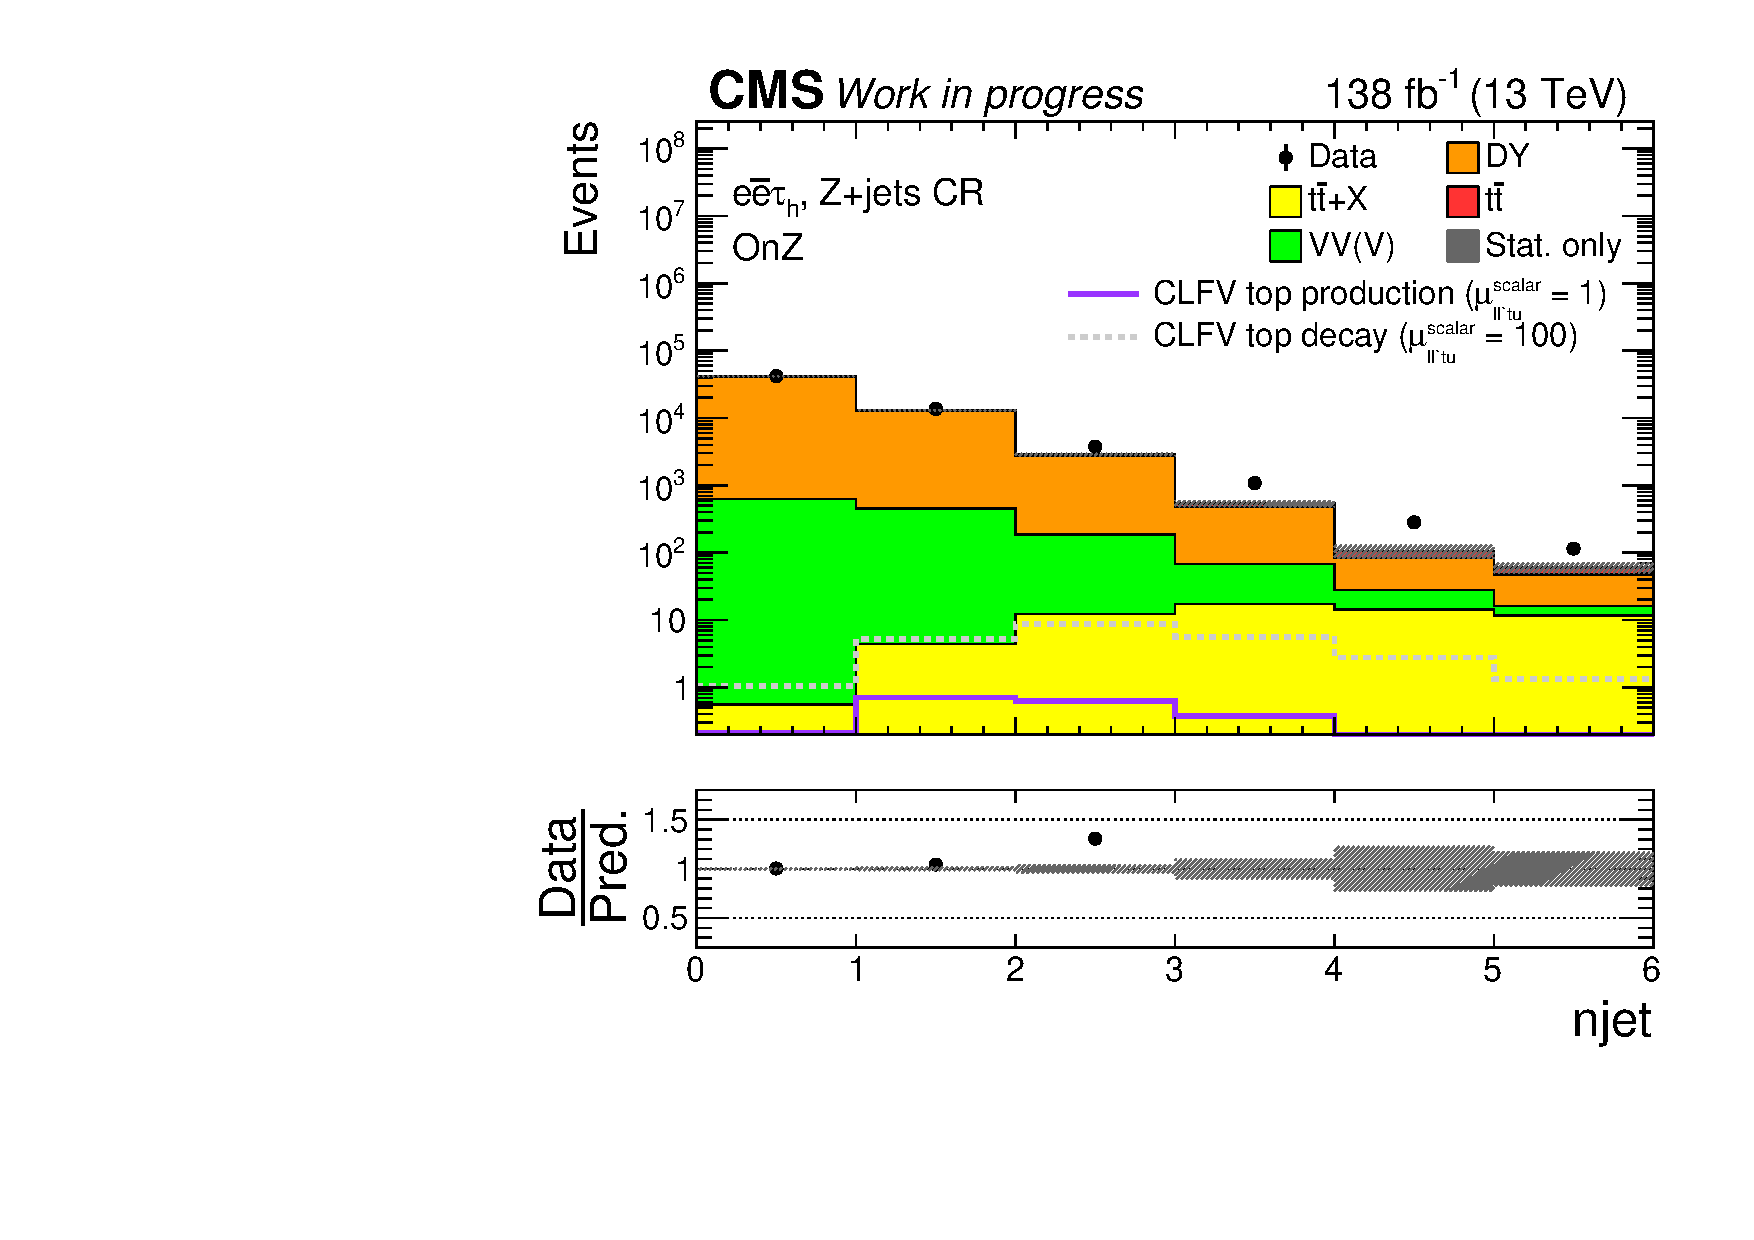
\includegraphics[width=0.48\textwidth]{figures/Part4/Evt/njet_OnZ_ee}&
 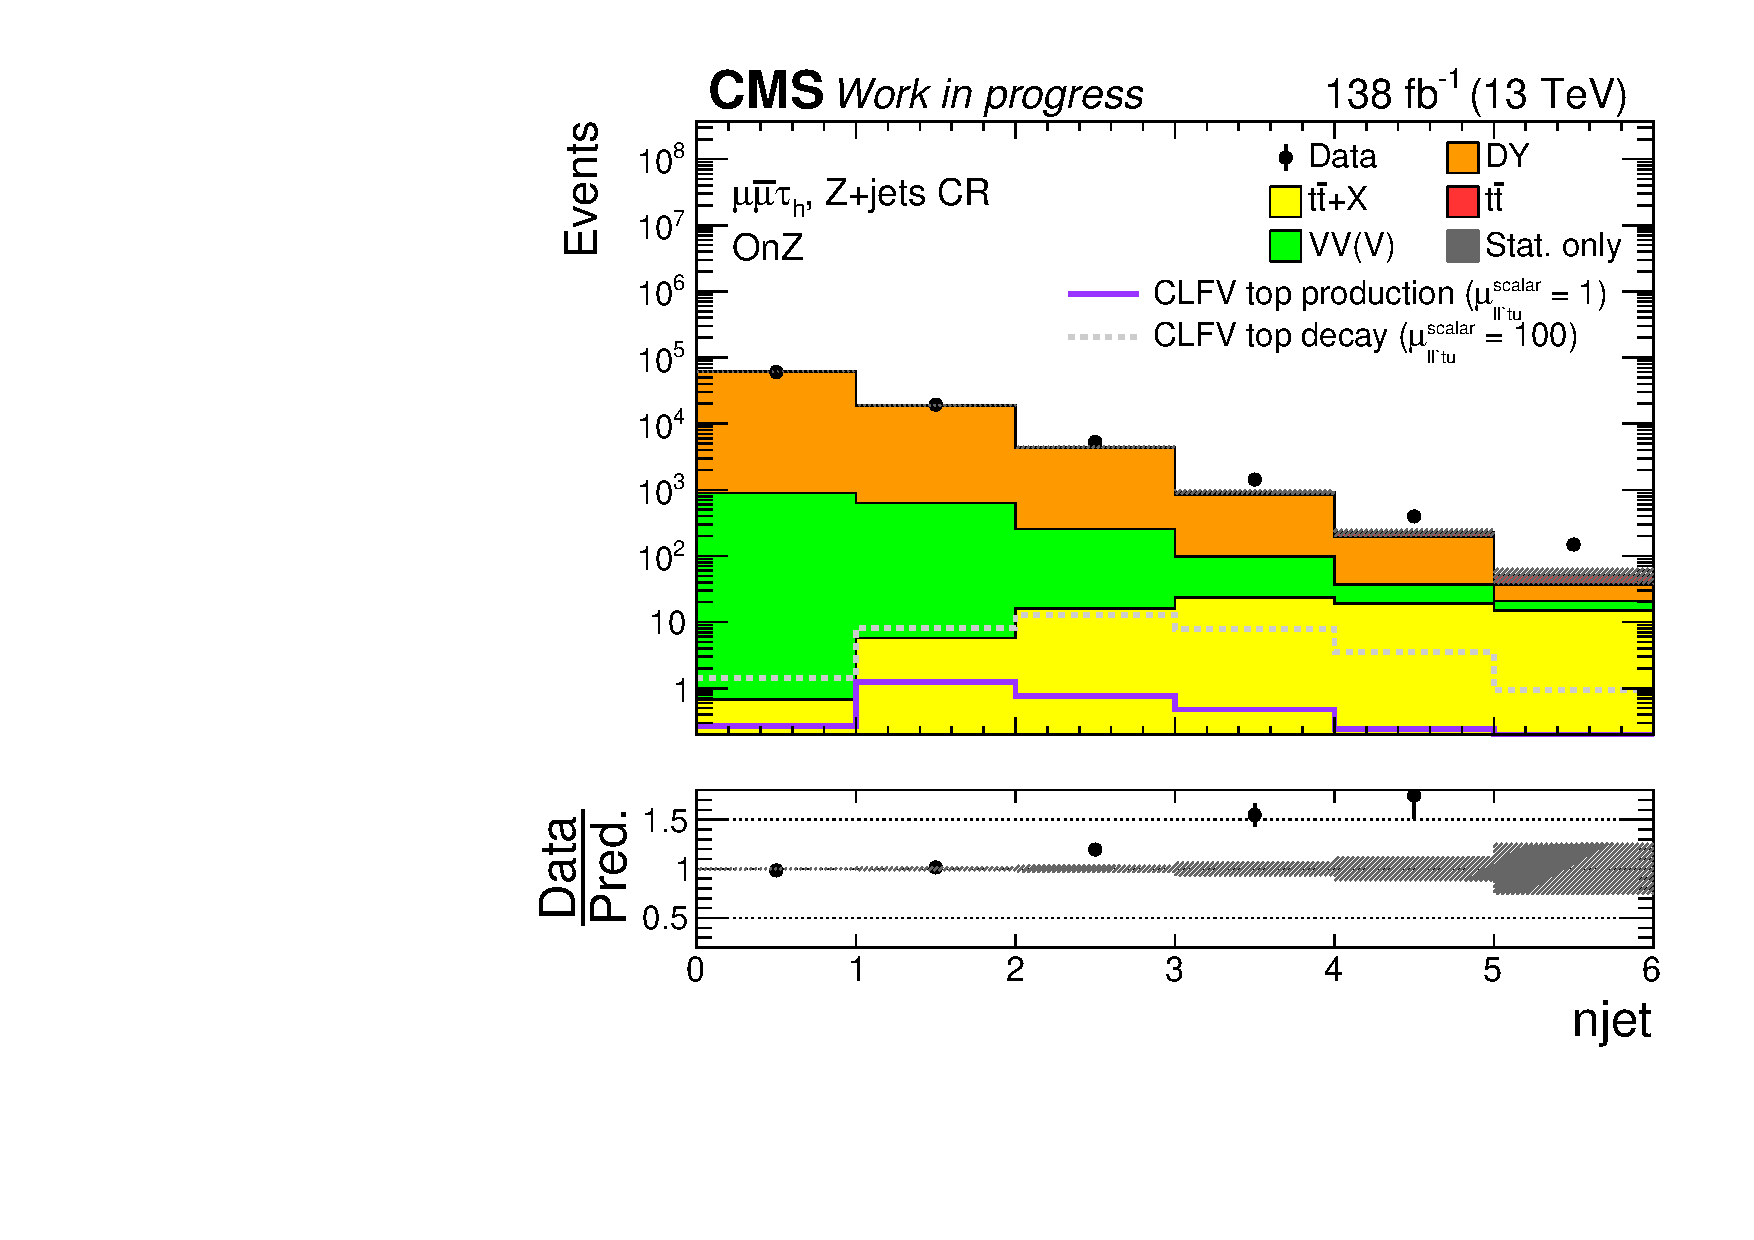
\includegraphics[width=0.48\textwidth]{figures/Part4/Evt/njet_OnZ_mumu}\\
 \end{tabular}
 \caption{XX}
 \label{fig:DY_CR}
 \end{center}
 \end{figure}